\documentclass{beamer}
\usetheme{Boadilla}

\usepackage{graphicx}
\usepackage{subcaption}
\usepackage{csvsimple}

% Change size of footnotes
\renewcommand{\footnotesize}{\fontsize{5pt}{5pt}\selectfont}
\title{Analysis of gene regulatory properties underlying trait pleiotropy}
\subtitle{Meeting GOLD 2022}
\author{Aitor Gonz\'alez}
\institute{Aix Marseille Univ, INSERM, TAGC}
\date{Oct. 19, 2022}

% Add section slide
\AtBeginSection[]
{
\begin{frame}
\frametitle{Table of Contents}
\tableofcontents[currentsection]
\end{frame}
}

\begin{document}

%%%%%%%%%%%%%%%%%%%%%%%%%%%%%%%%%%%%%%%%%%%%%%%%%%%%%%%%%%%%%%%%%%%%%%%%%%%%%%%%
\begin{frame}

\titlepage

\end{frame}


\section{Introduction} %%%%%%%%%%%%%%%%%%%%%%%%%%%%%%%%%%%%%%%%%%%%%%%%%%%%%%%%%%%%%%

%%%%%%%%%%%%%%%%%%%%%%%%%%%%%%%%%%%%%%%%%%%%%%%%%%%%%%%%%%%%%%%%%%%%%%%%%%%%%%%%
\begin{frame}
\frametitle{Genome-wide association studies (GWAS)}

\begin{itemize}
\item Genetic loci with higher frequency in individuals with a given disease
\item A very active field with many studies
\item Many genetic variants are involved in several phenotypes
\end{itemize}

\end{frame}

%%%%%%%%%%%%%%%%%%%%%%%%%%%%%%%%%%%%%%%%%%%%%%%%%%%%%%%%%%%%%%%%%%%%%%%%%%%%%%%%
\begin{frame}
\frametitle{Limitations of GWAS}

\begin{figure}[!]
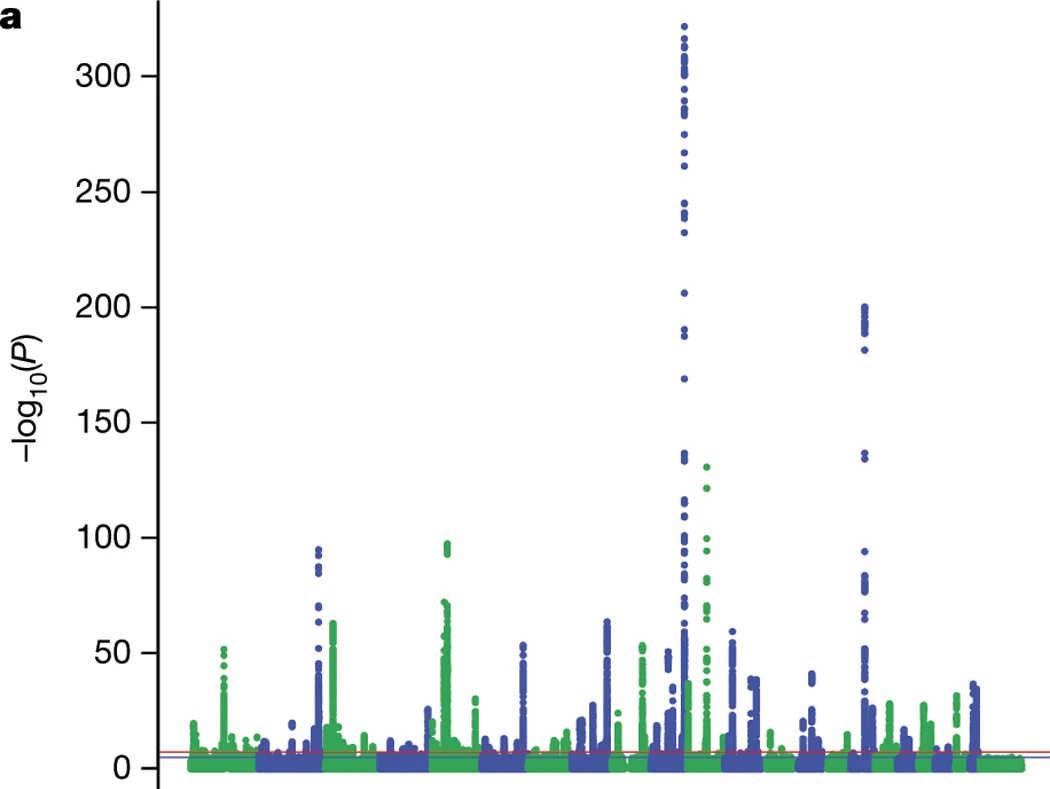
\includegraphics[width=0.25\textwidth]{/home/gonzalez/Repositories/gwas2eqtl_pleiotropy/presentation_gold2022_paris/fig/41586_2017_Article_BFnature24284_Fig1_HTML.jpg}
\caption{GWAS for breast cancer}
\end{figure}

\begin{itemize}
\item Correlation between variants, ie. LD
\item Which cell types are causal to the disease?
\item Over 90\% GWAS variants fall in non-coding regions
\end{itemize}
%
\vfill
%
These points can be partially addressed by looking at eQTLs in different tissues

\let\thefootnote\relax\footnotetext{doi:10.3389/fgene.2020.00424}
\end{frame}

%%%%%%%%%%%%%%%%%%%%%%%%%%%%%%%%%%%%%%%%%%%%%%%%%%%%%%%%%%%%%%%%%%%%%%%%%%%%%%%%
\begin{frame}
\frametitle{Integration of GWAS and eQTL variants:  Colocalisation analysis}

\begin{figure}[!]
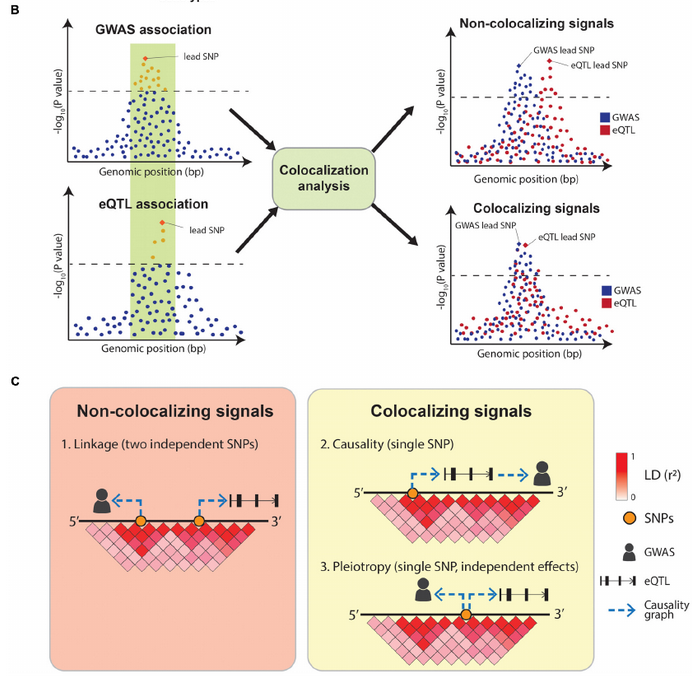
\includegraphics[width=0.6\textwidth]{/home/gonzalez/Repositories/gwas2eqtl_pleiotropy/presentation_gold2022_paris/fig/doi_10.3389_fgene.2020.00424_fig4.png}
\end{figure}

\let\thefootnote\relax\footnotetext{Cano-Gamez et al. 2020. doi:10.3389/fgene.2020.00424}
\end{frame}


\section{Objectives} %%%%%%%%%%%%%%%%%%%%%%%%%%%%%%%%%%%%%%%%%%%%%%%%%%%%%%%%%%%%%%

%%%%%%%%%%%%%%%%%%%%%%%%%%%%%%%%%%%%%%%%%%%%%%%%%%%%%%%%%%%%%%%%%%%%%%%%%%%%%%%%
\begin{frame}
\frametitle{Objectives}

\begin{itemize}
\item To carry out a large scale colocalization analysis between GWAS and eQTL variants
\item To identify pleiotropic genetic loci
\item To characterize the regulatory causas of this pleiotropy
\end{itemize}
\end{frame}

\section{Materials and Methods}

%%%%%%%%%%%%%%%%%%%%%%%%%%%%%%%%%%%%%%%%%%%%%%%%%%%%%%%%%%%%%%%%%%%%%%%%%%%%%%%%
\begin{frame}
\frametitle{Data and Algorithm}

\begin{itemize}
\item IEA OpenGWAS database
\item EBI eQTLs database
\item CRAN - Package coloc
\end{itemize}

\let\thefootnote\relax\footnotetext{https://gwas.mrcieu.ac.uk}
\end{frame}


\section{Results}

%%%%%%%%%%%%%%%%%%%%%%%%%%%%%%%%%%%%%%%%%%%%%%%%%%%%%%%%%%%%%%%%%%%%%%%%%%%%%%%%
\begin{frame}
\frametitle{Large scale GWAS/eQTL colocalization analysis}

\begin{itemize}
\item Colocalization of variants between 418 GWAS and 127 eQTL studies, ...
\end{itemize}

%\begin{figure}[!]
%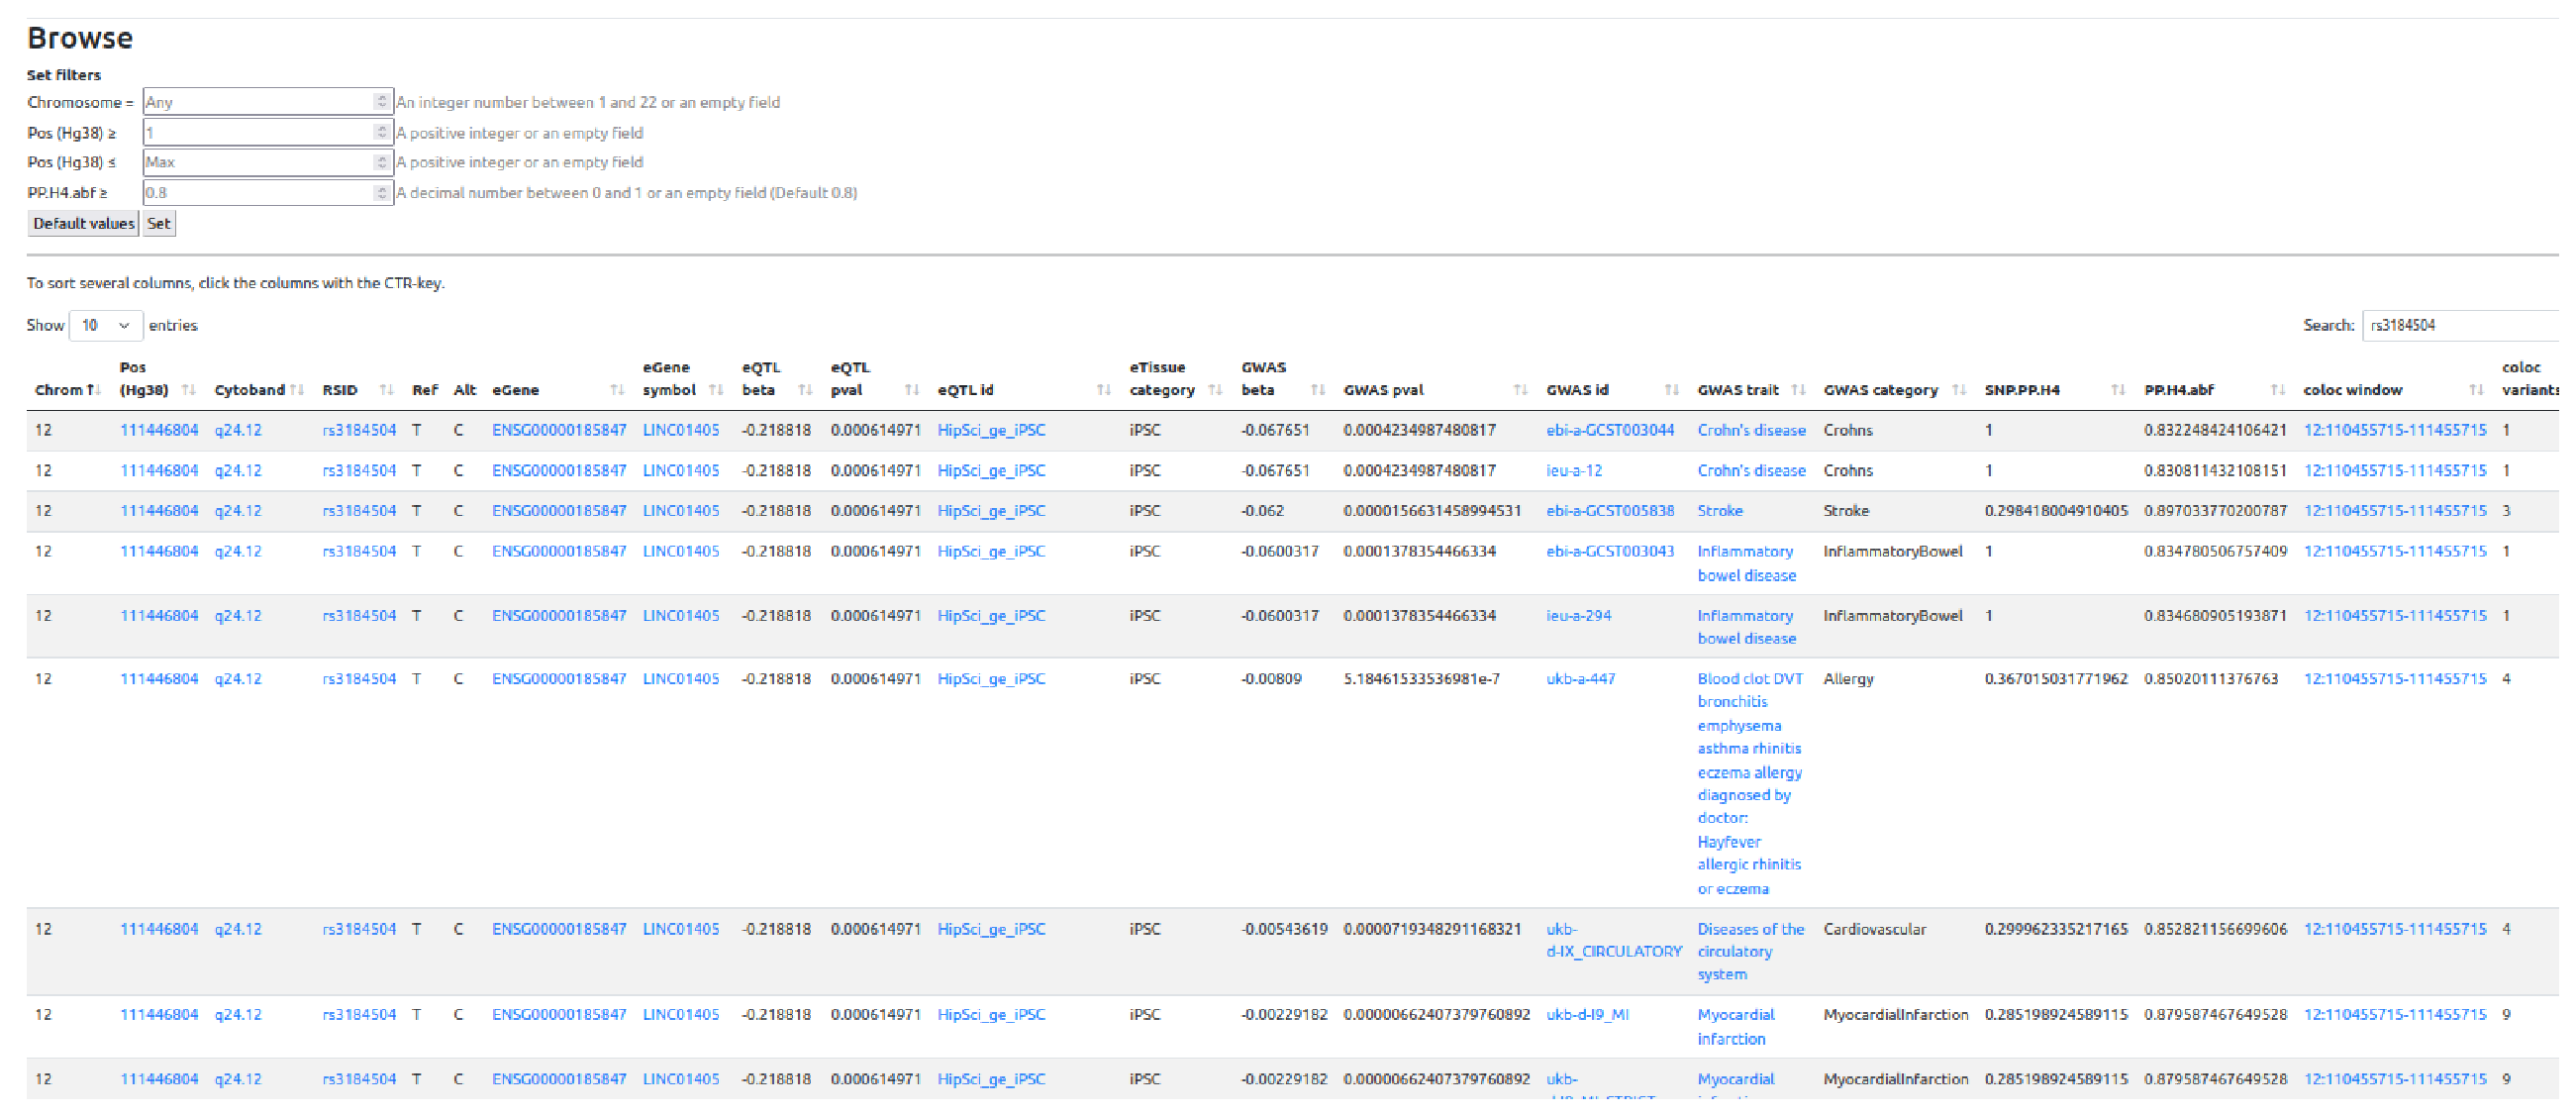
\includegraphics[width=0.6\textwidth]{/home/gonzalez/Repositories/gwas2eqtl_pleiotropy/poster_eccb22_barcelona/img/web.eps}
%\end{figure}

\end{frame}

%%%%%%%%%%%%%%%%%%%%%%%%%%%%%%%%%%%%%%%%%%%%%%%%%%%%%%%%%%%%%%%%%%%%%%%%%%%%%%%%
\begin{frame}
\frametitle{Do GWAS traits cluster coherently?}

\begin{itemize}
\item Distance between GWAS traits based on eQTL beta
\item Clustering of immune diseases coherent
\item eQTL beta of GWAS variants coherent
\end{itemize}

\begin{figure}[!]
\includegraphics[width=0.6\textwidth]{/home/gonzalez/Repositories/gwas2eqtl_pleiotropy/out/gwas418/pval_5e-08/r2_0.1/kb_1000/window_1000000/plthtmp_disease_comorbidity_matrix.py/corr.png}
\end{figure}

\end{frame}

%%%%%%%%%%%%%%%%%%%%%%%%%%%%%%%%%%%%%%%%%%%%%%%%%%%%%%%%%%%%%%%%%%%%%%%%%%%%%%%
%\begin{frame}
%\frametitle{Which are the most pleiotropic variants?}

%\begin{table}[!tbp]
%\centering
%\scriptsize
%\hline
%\csvreader[separator=tab,
%tabular=ccrrp{0.4\textwidth},
%head,
%table head=\bfseries Chrom. & \bfseries Cytoband & \bfseries Pos (hg38) & \bfseries Variant & \bfseries GWAS Categories\\\hline,
%]{/home/gonzalez/Repositories/gwas2eqtl_pleiotropy/out/gwas418/pval_5e-08/r2_0.1/kb_1000/window_1000000/cmpt_count_per_rsid.py/count_per_rsid_gwas_ms.tsv}{}% use head of csv as column names
%{\csvcoli\ & \csvcolii\ & \csvcoliii\ & \csvcoliv & \csvcolv}% specify your coloumns here
%\hline
%%
%\vspace{15pt}
%%
%\caption{Colocalized eQTL/GWAS variants involved in 5 or more GWAS categories. Genomic coordinates are given for the hg38 assembly. }\label{tab:pleitropic_variants}
%\end{table}

%\end{frame}


%%%%%%%%%%%%%%%%%%%%%%%%%%%%%%%%%%%%%%%%%%%%%%%%%%%%%%%%%%%%%%%%%%%%%%%%%%%%%%%%
\begin{frame}
\frametitle{Which are the most pleiotropic variants?}

\begin{itemize}
\item Distance between GWAS traits based on eQTL beta
\item Clustering of immune diseases coherent
\item eQTL beta of GWAS variants coherent
\end{itemize}

\begin{figure}[!]
\includegraphics[width=0.6\textwidth]{/home/gonzalez/Repositories/gwas2eqtl_pleiotropy/out/gwas418/pval_5e-08/r2_0.1/kb_1000/window_1000000/plthtmp_disease_comorbidity_matrix.py/corr.png}
\end{figure}

\end{frame}


%%%%%%%%%%%%%%%%%%%%%%%%%%%%%%%%%%%%%%%%%%%%%%%%%%%%%%%%%%%%%%%%%%%%%%%%%%%%%%%%
\begin{frame}
\frametitle{Do pleiotropic variants have more egenes?}

\begin{figure}[!tbp]
\centering
%
\begin{subfigure}[]{.32\textwidth}
\textbf{a}
\\
\includegraphics[width=\textwidth]{/home/gonzalez/Repositories/gwas2eqtl_pleiotropy/out/gwas418/pval_5e-08/r2_0.1/kb_1000/window_1000000/pltbar_x_per_variant_etissue_y_egene.py/plt.png}
\end{subfigure}
%
\begin{subfigure}[]{.32\textwidth}
\textbf{b}
\\
\includegraphics[width=\textwidth]{/home/gonzalez/Repositories/gwas2eqtl_pleiotropy/out/gwas418/pval_5e-08/r2_0.1/kb_1000/window_1000000/pltbar_x_per_variant_egene_y_etissue.py/plt.png}
\end{subfigure}
%
\begin{subfigure}[]{.32\textwidth}
\textbf{c}
\\
\includegraphics[width=\textwidth]{/home/gonzalez/Repositories/gwas2eqtl_pleiotropy/out/gwas418/pval_5e-08/r2_0.1/kb_1000/window_1000000/pltbar_x_per_variant_egene_etissue_y_gwas.py/plt.png}
\end{subfigure}
%
\caption{Count of eGenes per variant-tissue (\textbf{a}), eTissues per variant-eGene (\textbf{b}) and GWAS categories per variant-eGene-eTissue (\textbf{c}).} \label{fig:gwas_egene_etisue_per_variant}
%
\end{figure}

\end{frame}


\section{Conclusions, perspective and acknowledgements} %%%%%%%%%%%%%%%%%%%%%%%%%%%%%%%%%%%%%%%%%%%%%%%%%%%%%%%%%%%%%%

%%%%%%%%%%%%%%%%%%%%%%%%%%%%%%%%%%%%%%%%%%%%%%%%%%%%%%%%%%%%%%%%%%%%%%%%%%%%%%%%
\begin{frame}
\frametitle{Conclusions}

\begin{itemize}
\item A  colocalisation pipeline to link EBI Catalogue eQTLs and IEA OpenGWAS signals
\item Several colocalisation signals between immune cell eQTLs and cancer loci
\item Preliminary analyses of these colocalised signals
\end{itemize}

\end{frame}

%%%%%%%%%%%%%%%%%%%%%%%%%%%%%%%%%%%%%%%%%%%%%%%%%%%%%%%%%%%%%%%%%%%%%%%%%%%%%%%%
\begin{frame}
\frametitle{Perspectives}


\begin{itemize}
\item Use H1 as background dataset: H1=Causal SNP in cancer w/out eQTL
\item Statistics of cell type enrichments
\item Causal SNP characterization: Motif analyses
\item Other applications:
\begin{itemize}
\item Pleiotropy of eQTLs: eQTLs affecting two genes or same gene in two cell-types
\item Causality between other cell type eQTLs and diseases: Immunity and Covid-19
\end{itemize}
\end{itemize}

\end{frame}

%%%%%%%%%%%%%%%%%%%%%%%%%%%%%%%%%%%%%%%%%%%%%%%%%%%%%%%%%%%%%%%%%%%%%%%%%%%%%%%%
\begin{frame}
\frametitle{Acknowledgements}

\begin{itemize}
\item L\'eopoldine Lecerf (M1)
\item P Paul, P Rihet, M Michel
\item S Marquet, S Spicuglia
\item Funding:
\begin{itemize}
\item Institut Cancer et Immunologie (ICI)
\item Agence nationale de la recherche (ANR)
\end{itemize}
\end{itemize}

\end{frame}

\end{document}


